\let\negmedspace\undefined
\let\negthickspace\undefined
\documentclass[journal,12pt,onecolumn]{IEEEtran}
\usepackage{cite}
\usepackage{amsmath,amssymb,amsfonts,amsthm}
\usepackage{algorithmic}
\usepackage{graphicx}
\graphicspath{{./figs/}}
\usepackage{textcomp}
\usepackage{xcolor}
\usepackage{txfonts}
\usepackage{listings}
\usepackage{enumitem}
\usepackage{mathtools}
\usepackage{gensymb}
\usepackage{comment}
\usepackage{caption}
\usepackage[breaklinks=true]{hyperref}
\usepackage{tkz-euclide} 
\usepackage{listings}
\usepackage{gvv}                                        
%\def\inputGnumericTable{}                                 
\usepackage[latin1]{inputenc}     
\usepackage{xparse}
\usepackage{color}                                            
\usepackage{array}                                            
\usepackage{longtable}                                       
\usepackage{calc}                                             
\usepackage{multirow}
\usepackage{multicol}
\usepackage{hhline}                                           
\usepackage{ifthen}                                           
\usepackage{lscape}
\usepackage{tabularx}
\usepackage{array}
\usepackage{float}
\newtheorem{theorem}{Theorem}[section]
\newtheorem{problem}{Problem}
\newtheorem{proposition}{Proposition}[section]
\newtheorem{lemma}{Lemma}[section]
\newtheorem{corollary}[theorem]{Corollary}
\newtheorem{example}{Example}[section]
\newtheorem{definition}[problem]{Definition}
\newcommand{\BEQA}{\begin{eqnarray}}
\newcommand{\EEQA}{\end{eqnarray}}
\newcommand{\define}{\stackrel{\triangle}{=}}
\theoremstyle{remark}
\newtheorem{rem}{Remark}


\begin{document}

\title{
ASSIGNMENT 1: GATE 2008\\
GG : Geology and Geophysics}
\author{EE25BTECH11003 -Adharvan Kshathriya Bommagani}
\maketitle
\renewcommand{\thefigure}{\theenumi}
\renewcommand{\thetable}

\begin{enumerate}
    \item The planet having density less than $1.0~\text{gm/cm}^3$ is

    \hfill{\brak{\text{GATE GG 2008}}}
    
    \begin{multicols}{4}
        \begin{enumerate}
            \item Jupiter
            \item Neptune
            \item Saturn
            \item Uranus
        \end{enumerate}
    \end{multicols}

    \item Which mineral in a metamorphic rock indicates high grade metamorphism?

    \hfill{\brak{\text{GATE GG 2008}}}
    
    \begin{multicols}{2}
        \begin{enumerate}
            \item Chlorite
            \item Muscovite
            \item Serpentine
            \item Sillimanite
        \end{enumerate}
    \end{multicols}

    \item Which of the following landforms is formed by organisms?

    \hfill{\brak{\text{GATE GG 2008}}}
    
    \begin{multicols}{4}
        \begin{enumerate}
            \item Atoll
            \item Drumlins
            \item Outwash
            \item Point bar
        \end{enumerate}
    \end{multicols}

    \item The age of the sandstone reservoir in Cambay basin is

    \hfill{\brak{\text{GATE GG 2008}}}
    
    \begin{multicols}{4}
        \begin{enumerate}
            \item Cretaceous
            \item Eocene
            \item Holocene
            \item Jurassic
        \end{enumerate}
    \end{multicols}

    \item Due to Coriolis effect, the ocean currents will be deflected towards the right in

    \hfill{\brak{\text{GATE GG 2008}}}
    
    \begin{multicols}{2}
        \begin{enumerate}
            \item Antarctica
            \item Equator
            \item Southern Hemisphere
            \item Northern Hemisphere
        \end{enumerate}
    \end{multicols}

    \item The age of the Precambrian - Cambrian boundary \brak{\text{in million years}} is close to

    \hfill{\brak{\text{GATE GG 2008}}}
    
    \begin{multicols}{4}
        \begin{enumerate}
            \item 250
            \item 550
            \item 1550
            \item 2550
        \end{enumerate}
    \end{multicols}

    \item Which of the following minerals is harder than a knife blade?

    \hfill{\brak{\text{GATE GG 2008}}}
    
    \begin{multicols}{4}
        \begin{enumerate}
            \item Calcite
            \item Fluorite
            \item Gypsum
            \item Quartz
        \end{enumerate}
    \end{multicols}

    \item Choose a Proterozoic stratigraphic unit from the following

    \hfill{\brak{\text{GATE GG 2008}}}
    
    \begin{multicols}{2}
        \begin{enumerate}
            \item Cuddapah Super Group
            \item Dharwar Super Group
            \item Gondwana Super Group
            \item Iron Ore Group
        \end{enumerate}
    \end{multicols}

\newpage

    \item The correct pair of naturally occurring fissile isotope of Uranium is

    \hfill{\brak{\text{GATE GG 2008}}}
    
    \begin{multicols}{2}
        \begin{enumerate}
            \item $U^{236}$ and $U^{237}$
            \item $U^{235}$ and $U^{236}$
            \item $U^{235}$ and $U^{238}$
            \item $U^{236}$ and $U^{238}$
        \end{enumerate}
    \end{multicols}

    \item In the plate tectonic theory, the "ring of fire" around the Pacific ocean is related to

    \hfill{\brak{\text{GATE GG 2008}}}
    
    \begin{multicols}{2}
        \begin{enumerate}
            \item convergent plate boundary
            \item divergent plate boundary
            \item hot spots
            \item transform fault
        \end{enumerate}
    \end{multicols}

    \item The shear wave is

    \hfill{\brak{\text{GATE GG 2008}}}
    
    \begin{multicols}{2}
        \begin{enumerate}
            \item longitudinal
            \item dilatational
            \item irrotational
            \item equivoluminal
        \end{enumerate}
    \end{multicols}

    \item The liquid used in the sensor of a Proton Precession Magnetometer should be rich in

    \hfill{\brak{\text{GATE GG 2008}}}
    
    \begin{multicols}{4}
        \begin{enumerate}
            \item carbon
            \item hydrogen
            \item nitrogen
            \item oxygen
        \end{enumerate}
    \end{multicols}

    \item The dominant process of heat transport in the lithosphere is

    \hfill{\brak{\text{GATE GG 2008}}}
    
    \begin{multicols}{2}
        \begin{enumerate}
            \item advection
            \item conduction
            \item convection
            \item radiation
        \end{enumerate}
    \end{multicols}

    \item The shape of a vertical electric sounding curve over a three layer sequence comprising moist soil \brak{\text{top}}, fresh water saturated coarse sand \brak{\text{middle}} and clay \brak{\text{bottom}} is

    \hfill{\brak{\text{GATE GG 2008}}}
    
    \begin{multicols}{4}
        \begin{enumerate}
            \item A-type
            \item H-type
            \item K-type
            \item Q-type
        \end{enumerate}
    \end{multicols}

    \item The geophysical method that provided a convincing evidence of sea floor spreading is

    \hfill{\brak{\text{GATE GG 2008}}}
    
    \begin{multicols}{4}
        \begin{enumerate}
            \item gravity
            \item magnetic
            \item electric
            \item seismic
        \end{enumerate}
    \end{multicols}

    \item The difference in the gravity value \brak{\text{in mgal}} between the equator and pole is close to

    \hfill{\brak{\text{GATE GG 2008}}}
    
    \begin{multicols}{4}
        \begin{enumerate}
            \item 3786
            \item 4586
            \item 5186
            \item 5986
        \end{enumerate}
    \end{multicols}

    \item With respect to the Earth-Moon axis, the tidal deformation of the Earth produced by the Moon has the shape of

    \hfill{\brak{\text{GATE GG 2008}}}
    
    \begin{multicols}{2}
        \begin{enumerate}
            \item oblate ellipse
            \item oblate ellipsoid
            \item prolate ellipse
            \item prolate ellipsoid
        \end{enumerate}
    \end{multicols}

    \item A successful combination of geophysical methods for exploration of kimberlite pipe is

    \hfill{\brak{\text{GATE GG 2008}}}
    
    \begin{multicols}{2}
        \begin{enumerate}
            \item gravity and radiometric
            \item magnetic and electromagnetic
            \item radiometric and magnetic
            \item radiometric and seismic
        \end{enumerate}
    \end{multicols}

    \item Liquid outer core is evidenced by shadow zone for direct P-wave in the epicentral distance of

    \hfill{\brak{\text{GATE GG 2008}}}
    
    \begin{multicols}{2}
        \begin{enumerate}
            \item $92^{\degree}-132^{\degree}$
            \item $92^{\degree}-142^{\degree}$
            \item $102^{\degree}-132^{\degree}$
            \item $102^{\degree}-142^{\degree}$
        \end{enumerate}
    \end{multicols}

    \item Rift valleys are bounded by

    \hfill{\brak{\text{GATE GG 2008}}}
    
    \begin{multicols}{2}
        \begin{enumerate}
            \item normal faults
            \item reverse faults
            \item strike-slip faults
            \item transform faults
        \end{enumerate}
    \end{multicols}

    \item The composition of a sandstone is as follows: Quartz: 55\%, Feldspar: 25\%, Rock fragments: 1\% and Matrix: 19\%. Petrographically, the sandstone is classified as

    \hfill{\brak{\text{GATE GG 2008}}}
    
    \begin{multicols}{2}
        \begin{enumerate}
            \item arkose
            \item arkosic wacke
            \item lithic arenite
            \item quartz wacke
        \end{enumerate}
    \end{multicols}

    \item Match the sedimentary structures in Group I with the geological processes in Group II.

    \hfill{\brak{\text{GATE GG 2008}}}
    
    \begin{tabular}{ll}
        \textbf{Group I} & \textbf{Group II} \\
        P. Load casts & 1. Turbulent scour \\
        Q. Cross bedding & 2. Melting ice \\
        R. Flutes & 3. Soft sediment deformation \\
        S. Dropstones & 4. Biogenic \\
        & 5. Migration of mega ripples \\
    \end{tabular}
    
    \begin{multicols}{2}
        \begin{enumerate}
            \item P-3, Q-2, R-1, S-4
            \item P-2, Q-1, R-5, S-4
            \item P-3, Q-5, R-1, S-2
            \item P-1, Q-4, R-5, S-2
        \end{enumerate}
    \end{multicols}

    \item The phyllodes developed in echinoids to

    \hfill{\brak{\text{GATE GG 2008}}}
    
    \begin{multicols}{1}
        \begin{enumerate}
            \item increase efficiency in food collection
            \item protect it from sinking in muddy substratum
            \item burrow deep into the sediments
            \item protect it from predators
        \end{enumerate}
    \end{multicols}

    \item Two rock samples, P and Q, are characterized by the following well-preserved fossil assemblages: \\
    P: abundance of planktonic foraminifera and radiolaria \\
    Q: abundance of spore, pollen and vertebrate fossils \\
    Which of the following statements is true about the palaeoenvironmental conditions of the rocks?

    \hfill{\brak{\text{GATE GG 2008}}}
    
    \begin{multicols}{1}
        \begin{enumerate}
            \item P is estuarine and Q is deep marine
            \item P is inter-tidal and Q is terrestrial
            \item P is terrestrial and Q is shallow marine
            \item P is deep marine and Q is terrestrial
        \end{enumerate}
    \end{multicols}

    \item The evidence of Turonian marine transgression in Peninsular India is

    \hfill{\brak{\text{GATE GG 2008}}}
    
    \begin{multicols}{2}
        \begin{enumerate}
            \item Bagh Beds
            \item Niniyur Formation
            \item Patcham Formation
            \item Umaria Marine Bed
        \end{enumerate}
    \end{multicols}

    \item Match the stratigraphic units of India with their age:

    \hfill{\brak{\text{GATE GG 2008}}}
    
    \begin{tabular}{ll}
        \textbf{Stratigraphic Units} & \textbf{Age} \\
        P. Sargur Schist & 1. Oligocene \\
        Q. Kopili Shales & 2. Eocene \\
        R. Damuda Group & 3. Permian \\
        S. Kolhan Group & 4. Carboniferous \\
        & 5. Proterozoic \\
        & 6. Archaean \\
    \end{tabular}
    
    \begin{multicols}{2}
        \begin{enumerate}
            \item P-5, Q-3, R-4, S-1
            \item P-4, Q-3, R-1, S-5
            \item P-6, Q-1, R-2, S-5
            \item P-6, Q-2, R-3, S-5
        \end{enumerate}
    \end{multicols}

    \item In the following depth - temperature profile the broken lines indicate geothermal gradients. The zone in which oil and gas are likely to be generated and trapped is

    \hfill{\brak{\text{GATE GG 2008}}}
    
    \begin{figure}[h!]
        \centering
        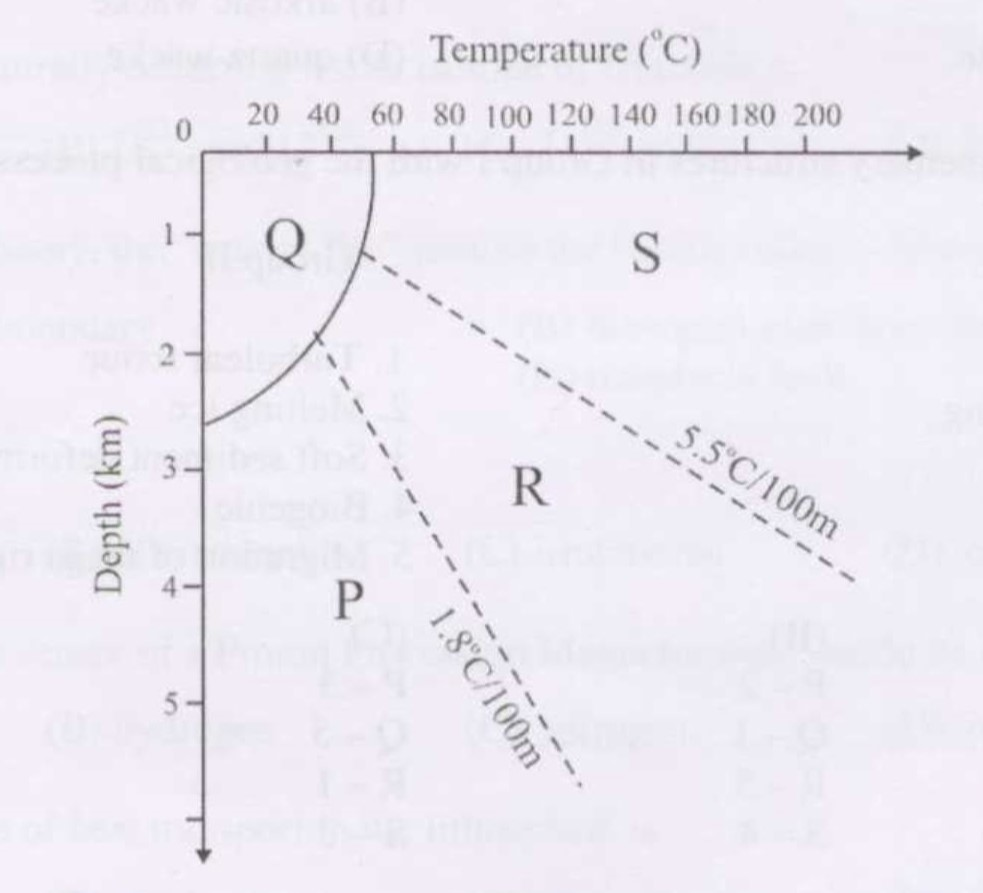
\includegraphics[width=0.4\textwidth]{figs/fig1.png}
        \caption{}
        \label{fig:q27}
    \end{figure}
    
    \begin{multicols}{4}
        \begin{enumerate}
            \item P
            \item Q
            \item R
            \item S
        \end{enumerate}
    \end{multicols}

    \item If a horizontal mirror plane is added to a pyramid having three-fold symmetry, the resultant symmetry of the c-axis will be

    \hfill{\brak{\text{GATE GG 2008}}}
    
    \begin{multicols}{4}
        \begin{enumerate}
            \item 3m
            \item $\overline{3}$
            \item $\overline{6}$
            \item $6/m$
        \end{enumerate}
    \end{multicols}

\newpage

    \item Dodecahedron and trapezohedron faces are observed in

    \hfill{\brak{\text{GATE GG 2008}}}
    
    \begin{multicols}{4}
        \begin{enumerate}
            \item beryl
            \item chalcopyrite
            \item fluorite
            \item garnet
        \end{enumerate}
    \end{multicols}

    \item The crystal system of biotite is

    \hfill{\brak{\text{GATE GG 2008}}}
    
    \begin{multicols}{4}
        \begin{enumerate}
            \item hexagonal
            \item monoclinic
            \item orthorhombic
            \item tetragonal
        \end{enumerate}
    \end{multicols}

    \item The \brak{\text{0001}} section of a uniaxial mineral can be distinguished from an isotropic mineral in thin section by

    \hfill{\brak{\text{GATE GG 2008}}}
    
    \begin{multicols}{2}
        \begin{enumerate}
            \item extinction angle
            \item pleochroism
            \item relief
            \item interference figure
        \end{enumerate}
    \end{multicols}

    \item Match the landforms in Group I with geomorphic processes in Group II

    \hfill{\brak{\text{GATE GG 2008}}}
    
    \begin{tabular}{ll}
        \textbf{Group I} & \textbf{Group II} \\
        P. Paired terrace & 1. Glacial erosion \\
        Q. Cirque & 2. Glacial deposition \\
        R. Barchan & 3. River rejuvenation \\
        S. Kames & 4. Wind erosion \\
        & 5. Wind deposition \\
    \end{tabular}
    
    \begin{multicols}{2}
        \begin{enumerate}
            \item P-4, Q-2, R-5, S-3
            \item P-2, Q-3, R-4, S-1
            \item P-3, Q-2, R-5, S-4
            \item P-3, Q-1, R-5, S-2
        \end{enumerate}
    \end{multicols}

    \item Match the ore/mineral deposits in Group I with genetic processes in Group II

    \hfill{\brak{\text{GATE GG 2008}}}
    
    \begin{tabular}{ll}
        \textbf{Group I} & \textbf{Group II} \\
        P. Kyanite & 1. Chemical sedimentation \\
        Q. Laterite & 2. Chemical weathering \\
        R. Banded iron ore & 3. Metamorphic \\
        S. Platinum & 4. Magmatic \\
    \end{tabular}
    
    \begin{multicols}{2}
        \begin{enumerate}
            \item P-2, Q-1, R-3, S-4
            \item P-3, Q-2, R-1, S-4
            \item P-4, Q-3, R-2, S-1
            \item P-3, Q-2, R-4, S-1
        \end{enumerate}
    \end{multicols}

    \item The scale of an aerial photograph acquired from a height of 5000 m using a camera having focal length of 200 mm, is

    \hfill{\brak{\text{GATE GG 2008}}}
    
    \begin{multicols}{4}
        \begin{enumerate}
            \item 1:5000
            \item 1:20000
            \item 1:40000
            \item 1:60000
        \end{enumerate}
    \end{multicols}

    \item The ratio of axial stress to corresponding axial strain for elastic material is known as

    \hfill{\brak{\text{GATE GG 2008}}}
    
    \begin{multicols}{2}
        \begin{enumerate}
            \item Bulk modulus
            \item Poisson's ratio
            \item Shear modulus
            \item Young's modulus
        \end{enumerate}
    \end{multicols}

\newpage

    \item An x-ray beam of wavelength $\lambda=1.541~\AA$ is incident on a cubic crystal having lattice spacing of 4 $\AA$. What will be its $2\theta$ value \brak{\text{where $\theta$ is the glancing angle}} on x-ray diffractogram?

    \hfill{\brak{\text{GATE GG 2008}}}
    
    \begin{multicols}{2}
        \begin{enumerate}
            \item $11.10^{\degree}$
            \item $20.10^{\degree}$
            \item $22.20^{\degree}$
            \item $44.20^{\degree}$
        \end{enumerate}
    \end{multicols}

    \item The dip slip of a fault is 200 m and the dip amount is 30$^{\degree}$. The throw of the fault \brak{\text{m}} is

    \hfill{\brak{\text{GATE GG 2008}}}
    
    \begin{multicols}{4}
        \begin{enumerate}
            \item 300
            \item 200
            \item 100
            \item 50
        \end{enumerate}
    \end{multicols}

    \item Which of the following modes of origin applies to snowball garnet?

    \hfill{\brak{\text{GATE GG 2008}}}
    
    \begin{multicols}{2}
        \begin{enumerate}
            \item Pre-tectonic
            \item Syn-tectonic
            \item Post-tectonic
            \item Contact metamorphic
        \end{enumerate}
    \end{multicols}

    \item Rocks of which of the following facies form under low geothermal gradient?

    \hfill{\brak{\text{GATE GG 2008}}}
    
    \begin{multicols}{2}
        \begin{enumerate}
            \item Blueschist
            \item Granulite
            \item Hornblende hornfels
            \item Sanidinite
        \end{enumerate}
    \end{multicols}

    \item Which of the following statements is/are true for porosity of sandstone? 

    \begin{enumerate}
    \item P - Porosity increases with sorting of grains. 
    \item Q - Porosity decreases with sorting of grains. 
    \item R - Porosity decreases with shale content. 
    \item S - Porosity increases with shale content.   
    \end{enumerate}

    \hfill{\brak{\text{GATE GG 2008}}}
    
    \begin{multicols}{4}
        \begin{enumerate}
            \item Q
            \item P, S
            \item P, R
            \item S
        \end{enumerate}
    \end{multicols}

    \item On crystallization of anorthite, Sr concentration in the magma will

    \hfill{\brak{\text{GATE GG 2008}}}
    
    \begin{multicols}{2}
        \begin{enumerate}
            \item decrease
            \item increase
            \item increase and then decrease
            \item remain constant
        \end{enumerate}
    \end{multicols}

    \item If the solubility product of gypsum is $10^{-4.36}$, the solubility \brak{\text{mol/litre}} of gypsum in an ideal aqueous solution will be

    \hfill{\brak{\text{GATE GG 2008}}}
    
    \begin{multicols}{2}
        \begin{enumerate}
            \item $10^{-9.72}$
            \item $10^{-4.36}$
            \item $10^{-2.18}$
            \item $10^{-1.09}$
        \end{enumerate}
    \end{multicols}

    \item What is the age of the lignite deposit of Neyveli?

    \hfill{\brak{\text{GATE GG 2008}}}
    
    \begin{multicols}{4}
        \begin{enumerate}
            \item Eocene
            \item Miocene
            \item Oligocene
            \item Permian
        \end{enumerate}
    \end{multicols}

\newpage

    \item Find the correct match of mineral pair in Group I with the corresponding crystallization behaviour in Group II

    \hfill{\brak{\text{GATE GG 2008}}}
    
    \begin{tabular}{ll}
        \textbf{Group I} & \textbf{Group II} \\
        P. Silica K feldspar & 1. Solid solution \\
        Q. Albite Anorthite & 2. Peritectic \\
        R. Forsterite - Silica & 3. Eutectic \\
    \end{tabular}
    
    \begin{multicols}{2}
        \begin{enumerate}
            \item P-3, Q-1, R-2
            \item P-1, Q-2, R-3
            \item P-2, Q-1, R-3
            \item P-3, Q-2, R-1
        \end{enumerate}
    \end{multicols}

    \item An igneous rock with 50\% olivine, 25\% orthopyroxene and 25\% clinopyroxene by mode will be called

    \hfill{\brak{\text{GATE GG 2008}}}
    
    \begin{multicols}{4}
        \begin{enumerate}
            \item dunite
            \item harzburgite
            \item lherzolite
            \item wehrlite
        \end{enumerate}
    \end{multicols}

    \item In a gravity survey, if the observation point lies below the datum plane, then for gravity data reduction

    \hfill{\brak{\text{GATE GG 2008}}}
    
    \begin{multicols}{1}
        \begin{enumerate}
            \item Free-air and Bouguer corrections are positive
            \item Free-air correction is positive and Bouguer correction is negative
            \item Free-air correction is negative and Bouguer correction is positive
            \item Free-air and Bouguer corrections are negative
        \end{enumerate}
    \end{multicols}

    \item If the Earth's magnetic field at the north pole is 60,000 $\gamma$ and the radius of Earth is R, at what height above the north pole will its magnitude be 30,000 $\gamma$?

    \hfill{\brak{\text{GATE GG 2008}}}
    
    \begin{multicols}{4}
        \begin{enumerate}
            \item 0.26 R
            \item 0.52 R
            \item 0.78 R
            \item 1.04 R
        \end{enumerate}
    \end{multicols}

    \item Match the apparent resistivity type curves observed on the surface in Group I with the subsurface resistivity variations in Group II

    \hfill{\brak{\text{GATE GG 2008}}}
    
    \begin{tabular}{ll}
        \textbf{Group I} & \textbf{Group II} \\
        P. AK-Type & 1. $\rho_{1}<\rho_{2}>\rho_{3}>\rho_{4}$ \\
        Q. HK-Type & 2. $\rho_{1}>\rho_{2}<\rho_{3}>\rho_{4}$ \\
        R. KQ-Type & 3. $\rho_{1}>\rho_{2}<\rho_{3}<\rho_{4}$ \\
        S. HA-Type & 4. $\rho_{1}<\rho_{2}<\rho_{3}<\rho_{4}$ \\
        & 5. $\rho_{1}<\rho_{2}>\rho_{3}<\rho_{4}$ \\
        & 6. $\rho_{1}<\rho_{2}<\rho_{3}>\rho_{4}$ \\
    \end{tabular}
    
    \begin{multicols}{2}
        \begin{enumerate}
            \item P-2, Q-4, R-1, S-3
            \item P-3, Q-4, R-2, S-6
            \item P-4, Q-5, R-6, S-1
            \item P-6, Q-2, R-1, S-3
        \end{enumerate}
    \end{multicols}

\newpage

    \item The plane wave electromagnetic field traveling vertically downward in a homogeneous half-space of resistivity 500 $\Omega$m varies with depth 'z' as,
    \begin{align*}
    H_{y}(z)=H_{0}e^{-0.5z}\{\cos(\omega t-0.5z)+i~\sin(\omega t-0.5z)\}
    \end{align*}
    What is the frequency \brak{\text{in Hz}} of the primary field given $\mu=\mu_{0}=4\pi\times10^{-7}$ H/m?

    \hfill{\brak{\text{GATE GG 2008}}}
    
    \begin{multicols}{2}
        \begin{enumerate}
            \item $7.16\times10^{7}$
            \item $5.16\times10^{7}$
            \item $3.16\times10^{7}$
            \item $1.16\times10^{7}$
        \end{enumerate}
    \end{multicols}

    \item Wenner survey is performed over a homogeneous ground of resistivity 200 $\Omega$m. For the current electrode spacing of 60 m, 100 mA current flow is recorded. What will be the magnitude of potential difference \brak{\text{in mV}} between potential electrodes?

    \hfill{\brak{\text{GATE GG 2008}}}
    
    \begin{multicols}{2}
        \begin{enumerate}
            \item 53.0
            \item 159.2
            \item 477.7
            \item 1433.1
        \end{enumerate}
    \end{multicols}

    \item Potential Difference \brak{\text{PD}} and Gradient of Potential Difference \brak{\text{GPD}} are measured along a profile over a massive sulfide body in self-potential survey. Which of the following statements is correct for the anomalies over the center of the body?

    \hfill{\brak{\text{GATE GG 2008}}}
    
    \begin{multicols}{1}
        \begin{enumerate}
            \item PD is positive and GPD is positive
            \item PD is positive and GPD is zero
            \item PD is negative and GPD is negative
            \item PD is negative and GPD is zero
        \end{enumerate}
    \end{multicols}

    \item Match the phase differences between the quantities of induction phenomena \brak{\text{Group I}} with the amount of phase difference in Group II

    \hfill{\brak{\text{GATE GG 2008}}}
    
    \begin{tabular}{ll}
        \textbf{Group I} & \textbf{Group II} \\
        P. Secondary field with respect to primary field & 1. leads by $90^{\degree}$ \\
        Q. Inphase component of secondary field & 2. lags by $90^{\degree}$ \\
        \quad with respect to primary field & \\
        R. Quadrature component of secondary field & 3. lags between $90^{\degree}-180^{\degree}$ \\
        \quad with respect to primary field & \\
        S. Quadrature component of secondary field & 4. lags by $180^{\degree}$ \\
        \quad with respect to inphase component of secondary field & \\
    \end{tabular}
    
    \begin{multicols}{2}
        \begin{enumerate}
            \item P-4, Q-1, R-3, S-2
            \item P-1, Q-2, R-4, S-3
            \item P-2, Q-3, R-1, S-4
            \item P-3, Q-4, R-2, S-1
        \end{enumerate}
    \end{multicols}

    \item Which of the following combinations of electromagnetic field components is measured in magnetotelluric method?

    \hfill{\brak{\text{GATE GG 2008}}}
    
    \begin{multicols}{2}
        \begin{enumerate}
            \item $E_{x}, E_{y}, H_{x}, H_{y}, H_{z}$
            \item $E_{x}, E_{y}, E_{z}, H_{x}, H_{z}$
            \item $E_{x}, E_{y}, E_{z}, H_{y}, H_{z}$
            \item $E_{x}, E_{z}, H_{x}, H_{y}, H_{z}$
        \end{enumerate}
    \end{multicols}

\newpage

    \item Which form of partial differential equation is used for the interpretation of electromagnetic anomalies in geophysical prospecting?

    \hfill{\brak{\text{GATE GG 2008}}}
    
    \begin{multicols}{2}
        \begin{enumerate}
            \item Diffusion equation
            \item Laplace's equation
            \item Poisson's equation
            \item Wave equation
        \end{enumerate}
    \end{multicols}

    \item A radioactive substance decays to one third of its original value in 6 hours time. What is the half-life \brak{\text{in hours}} of the substance?

    \hfill{\brak{\text{GATE GG 2008}}}
    
    \begin{multicols}{4}
        \begin{enumerate}
            \item 3.58
            \item 3.78
            \item 3.98
            \item 4.18
        \end{enumerate}
    \end{multicols}

    \item The relation between magnetic latitude \brak{\text{$\theta$}} and the magnetic inclination \brak{\text{i}} is

    \hfill{\brak{\text{GATE GG 2008}}}
    
    \begin{multicols}{2}
        \begin{enumerate}
            \item $2 \tan i = \tan \theta$
            \item $\tan i = 2 \tan \theta$
            \item $\tan i = 2 \tan^{2}\theta$
            \item $2 \tan i = \cos \theta$
        \end{enumerate}
    \end{multicols}

    \item To derive magnetic field from gravity field, the Poisson's relation can be used only when the direction of magnetization is

    \hfill{\brak{\text{GATE GG 2008}}}
    
    \begin{multicols}{2}
        \begin{enumerate}
            \item horizontal \brak{\text{$0^{\degree}$}}
            \item $45^{\degree}$
            \item $60^{\degree}$
            \item vertical \brak{\text{$90^{\degree}$}}
        \end{enumerate}
    \end{multicols}

    \item Fourier analysis matches the signal by a series of sinusoids. Each member of the series fits an exact number of

    \hfill{\brak{\text{GATE GG 2008}}}
    
    \begin{multicols}{2}
        \begin{enumerate}
            \item one-fourth wavelength
            \item one-third wavelength
            \item half-wavelength
            \item one wavelength
        \end{enumerate}
    \end{multicols}

    \item Compton scattering is the physical basis of

    \hfill{\brak{\text{GATE GG 2008}}}
    
    \begin{multicols}{2}
        \begin{enumerate}
            \item Neutron - Gamma logging
            \item Neutron-thermal neutron logging
            \item Natural Gamma logging
            \item Gamma - Gamma logging
        \end{enumerate}
    \end{multicols}

    \item If the P-wave velocity is twice that of S-wave velocity in a medium, the Poisson's ratio of the material is

    \hfill{\brak{\text{GATE GG 2008}}}
    
    \begin{multicols}{4}
        \begin{enumerate}
            \item 0.50
            \item 0.33
            \item 0.25
            \item 0.12
        \end{enumerate}
    \end{multicols}

    \item The Lame's coefficient \brak{\text{$\lambda$}} can be written in terms of compressibility of the material \brak{\text{$\beta$}} and Poisson's ratio \brak{\text{$\sigma$}} as

    \hfill{\brak{\text{GATE GG 2008}}}
    
    \begin{multicols}{2}
        \begin{enumerate}
            \item $\lambda=\frac{3\sigma}{(1+\sigma)\beta}$
            \item $\lambda=\frac{(1+\sigma)}{3\sigma\beta}$
            \item $\lambda=\frac{\sigma}{(1+\sigma)(1-2\sigma)\beta}$
            \item $\lambda=\frac{3(1-2\sigma)}{\beta}$
        \end{enumerate}
    \end{multicols}

    \item The amplitude of seismic wave varies due to spherical spreading as a function of

    \hfill{\brak{\text{GATE GG 2008}}}
    
    \begin{multicols}{2}
        \begin{enumerate}
            \item radius of sphere
            \item 1/\brak{\text{radius of sphere}}
            \item \brak{\text{radius of sphere}}$^2$
            \item 1/\brak{\text{radius of sphere}}$^2$
        \end{enumerate}
    \end{multicols}

    \item If f is the frequency of seismic wave and v is its velocity, the relation between absorption coefficient \brak{\text{$\alpha$}} and quality factor \brak{\text{Q}} is

    \hfill{\brak{\text{GATE GG 2008}}}
    
    \begin{multicols}{2}
        \begin{enumerate}
            \item $\alpha=\frac{\pi f}{Qv}$
            \item $\alpha=\frac{Qf}{\pi v}$
            \item $\alpha=\frac{Qv}{\pi f}$
            \item $\alpha=\frac{\pi Q}{vf}$
        \end{enumerate}
    \end{multicols}

    \item In marine seismic surveys, the maximum depth d \brak{\text{in feet}} at which the bubble will break is related to the charge weight W \brak{\text{in pounds}} by the relation

    \hfill{\brak{\text{GATE GG 2008}}}
    
    \begin{multicols}{2}
        \begin{enumerate}
            \item $d=3.8~W$
            \item $d=3.8~W^{1/2}$
            \item $d=3.8~W^{1/3}$
            \item $d=3.8~W^{1/4}$
        \end{enumerate}
    \end{multicols}

    \item Considering noise problem \brak{\text{reverberation}} in marine seismic work, the frequencies for higher harmonics are expressed by $f_{n}=\frac{(2n-1)V_{w}}{4d_{w}}$, where $f_{n}$ - frequency of $n^{th}$ harmonic, $V_{w}$ - velocity of sound in water and $d_{w}$ - water depth. The fundamental frequency in terms of the reciprocal of one way travel time is

    \hfill{\brak{\text{GATE GG 2008}}}
    
    \begin{multicols}{2}
        \begin{enumerate}
            \item one - fourth
            \item one - third
            \item one - half
            \item three fourth
        \end{enumerate}
    \end{multicols}

    \item In a linear inverse problem having rectangular system matrix that is rank deficient, the inverse solution is

    \hfill{\brak{\text{GATE GG 2008}}}
    
    \begin{multicols}{2}
        \begin{enumerate}
            \item unique solution
            \item least square solution
            \item minimum norm solution
            \item minimum norm least square solution
        \end{enumerate}
    \end{multicols}

    \item In a linear inverse problem having eigenvalues 100, 10, 1, 0.1, 0.01, 0.001, the highest condition number of the system matrix is

    \hfill{\brak{\text{GATE GG 2008}}}
    
    \begin{multicols}{4}
        \begin{enumerate}
            \item 100000
            \item 10000
            \item 1000
            \item 100
        \end{enumerate}
    \end{multicols}

    \item A combination of radioactive logging to detect chlorine in a formation is

    \hfill{\brak{\text{GATE GG 2008}}}
    
    \begin{multicols}{1}
        \begin{enumerate}
            \item Neutron-thermal neutron log and Gamma-Gamma log
            \item Neutron-epithermal neutron log and Neutron-Gamma log
            \item Neutron-Gamma log and Gamma-Gamma log
            \item Neutron-epithermal neutron log and Gamma-Gamma log
        \end{enumerate}
    \end{multicols}

\newpage

    \item In electrical logging, the measured resistivity of flushed zone is 19.2 $\Omega$m, the resistivity of mud-filtrate is 1.33 $\Omega$m and the computed value of residual oil saturation in flushed zone is 20\%. The value of formation resistivity factor is

    \hfill{\brak{\text{GATE GG 2008}}}
    
    \begin{multicols}{4}
        \begin{enumerate}
            \item 8.50
            \item 8.85
            \item 9.11
            \item 9.24
        \end{enumerate}
    \end{multicols}

    \item In a seismic reflection survey, lithological boundaries P \brak{\text{Shale and Gas sand}}, Q \brak{\text{Gas sand and Oil sand}} and R \brak{\text{Oil sand and Water sand}} computed on the basis of reflection coefficients are shown in figure. Which is the correct sequence of reflection coefficients at these boundaries?

    \hfill{\brak{\text{GATE GG 2008}}}
    
    \begin{figure}[h!]
        \centering
        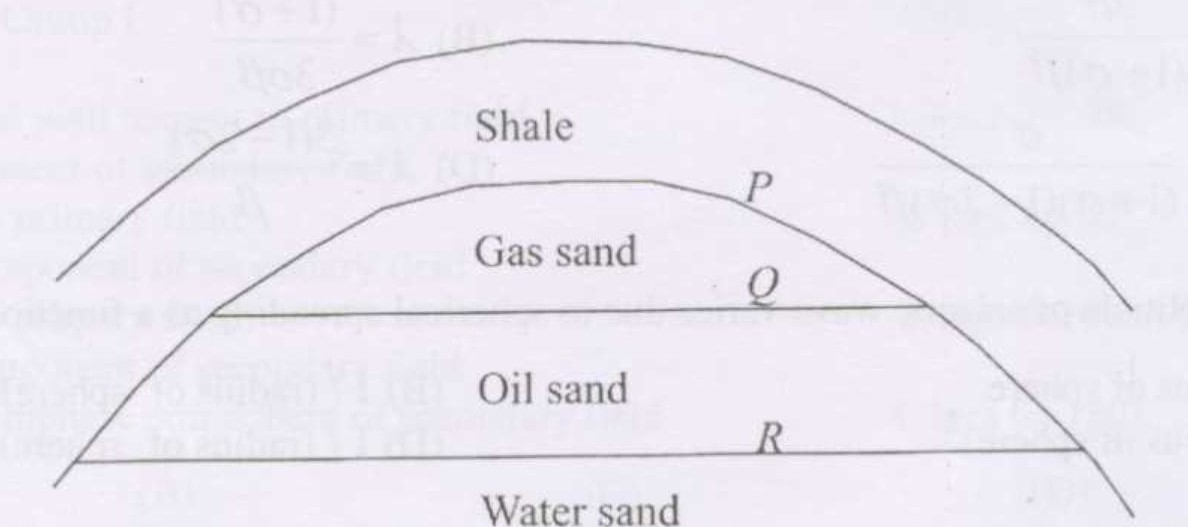
\includegraphics[width=0.4\textwidth]{figs/fig2.png}
        \caption{}
        \label{fig:q70}
    \end{figure}
    
    \begin{multicols}{2}
        \begin{enumerate}
            \item P \brak{\text{-0.30}}, Q \brak{\text{+0.20}}, R \brak{\text{+0.03}}
            \item P \brak{\text{-0.30}}, Q \brak{\text{+0.03}}, R \brak{\text{+0.20}}
            \item P \brak{\text{+0.20}}, Q \brak{\text{-0.30}}, R \brak{\text{+0.03}}
            \item P \brak{\text{+0.20}}, Q \brak{\text{+0.03}}, R \brak{\text{-0.30}}
        \end{enumerate}
    \end{multicols}



    \item[] \textbf{Common Data for Questions 71, 72 and 73:} The following geological map shows exposures of sedimentary beds p, q, r, s, t and a batholith \brak{\text{hatched}} in a flat terrain.
    
    \begin{figure}[h!]
        \centering
        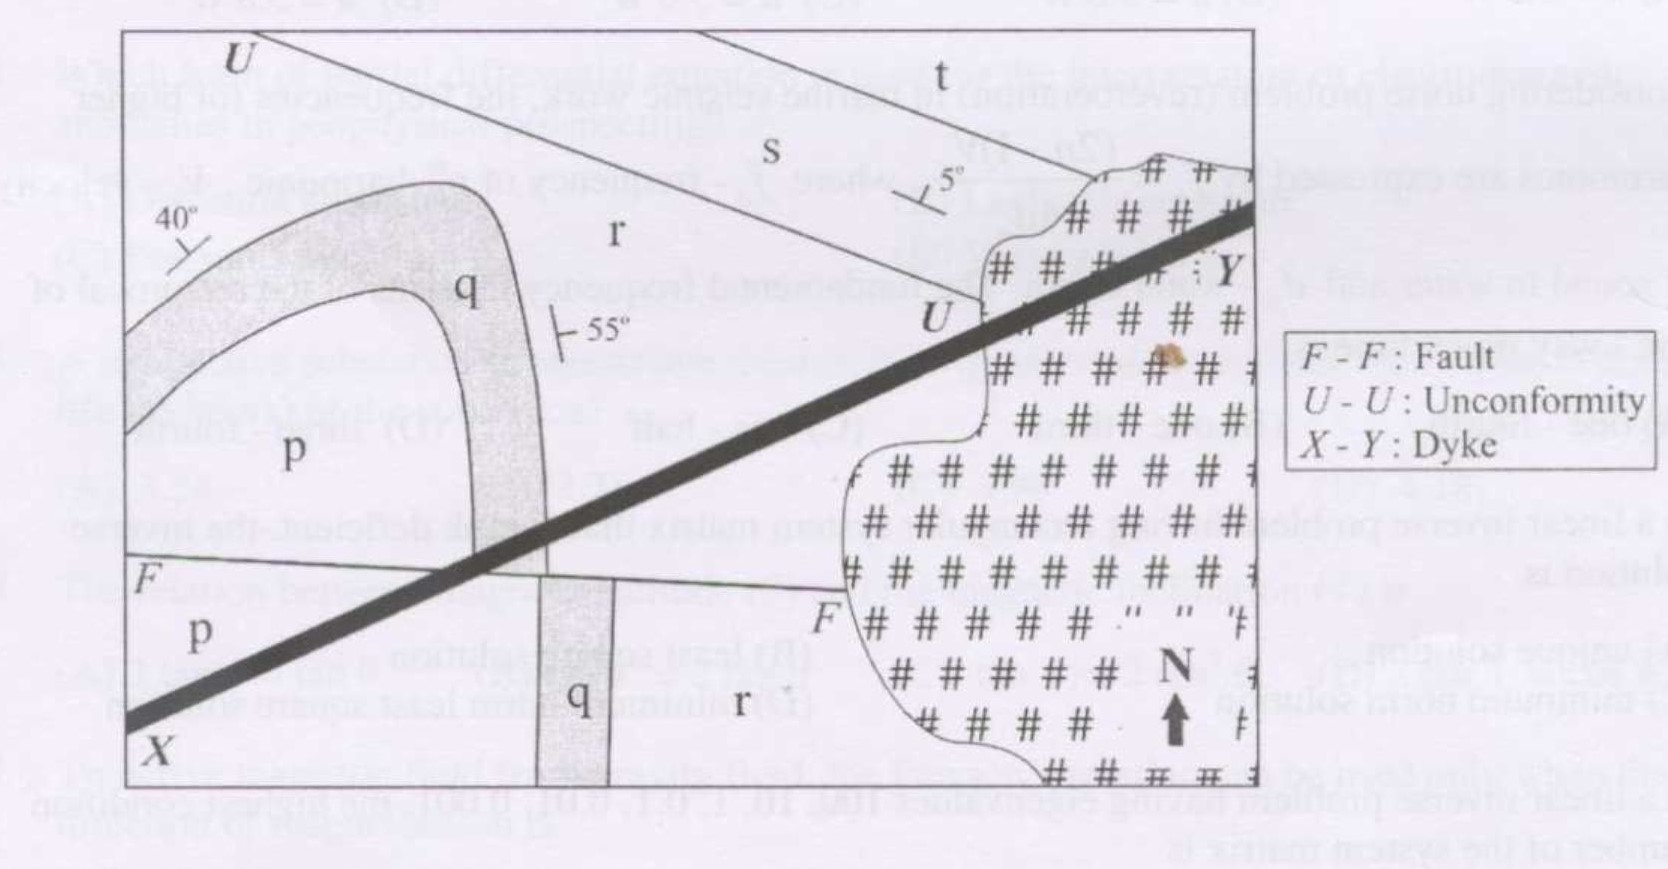
\includegraphics[width=0.4\textwidth]{figs/fig3.png}
        \caption{}
        \label{Fig.71-73}
    \end{figure}
    
    \item The fold seen in the area is 

    \hfill{\brak{\text{GATE GG 2008}}}
    
    \begin{multicols}{2}
        \begin{enumerate}
            \item a synform plunging northerly
            \item a synform plunging southerly
            \item an antiform plunging northerly
            \item an antiform plunging southerly
        \end{enumerate}
    \end{multicols}

    \item If the fault dips $70^{\degree}$ southerly, it is a

    \hfill{\brak{\text{GATE GG 2008}}}
    
    \begin{multicols}{2}
        \begin{enumerate}
            \item normal fault with southern upthrown block
            \item right lateral strike-slip fault
            \item reverse fault with northern upthrown block
            \item reverse fault with southern upthrown block
        \end{enumerate}
    \end{multicols}

\newpage

    \item The intrusion of dyke took place

    \hfill{\brak{\text{GATE GG 2008}}}
    
    \begin{multicols}{2}
        \begin{enumerate}
            \item after deposition of beds 's' and 't'
            \item before deposition of beds 's' and 't'
            \item before faulting
            \item before folding
        \end{enumerate}
    \end{multicols}

    \item[] \textbf{Common Data for Questions 74 and 75:} Two sampled data sets are given as: $X(t) = [1, \frac{1}{2}, -1, -\frac{1}{2}]$ and $Y(t) = [1, -\frac{1}{2}, -1, \frac{1}{2}]$.
    
    \item The cross-correlation between these two time series for zero lag is

    \hfill{\brak{\text{GATE GG 2008}}}
    
    \begin{multicols}{4}
        \begin{enumerate}
            \item $-\frac{3}{2}$
            \item $\frac{5}{2}$
            \item $-\frac{1}{2}$
            \item $\frac{3}{2}$
        \end{enumerate}
    \end{multicols}

    \item The convolution of the data sets results in a time series

    \hfill{\brak{\text{GATE GG 2008}}}
    
    \begin{multicols}{2}
        \begin{enumerate}
            \item $[1, 1, -\frac{11}{2}, 4, -\frac{17}{2}, -1, 1]$
            \item $[-1, 1, 4, \frac{17}{2}, -\frac{11}{2}, 1, 1]$
            \item $[1, \frac{17}{2}, 4, -\frac{11}{2}, -1, \frac{3}{2}, 1]$
            \item $[1, -1, \frac{17}{2}, 5, \frac{11}{2}, -1, 1]$
        \end{enumerate}
    \end{multicols}



    \item[] \textbf{Statement for Linked Answer Questions 76 and 77:} A mineral assemblage consists of fayalite, ferro-silite and quartz in equilibrium.
    
    \item The number of components in the system is

    \hfill{\brak{\text{GATE GG 2008}}}
    
    \begin{multicols}{4}
        \begin{enumerate}
            \item 4
            \item 1
            \item 2
            \item 3
        \end{enumerate}
    \end{multicols}

    \item The degree of freedom of the system is

    \hfill{\brak{\text{GATE GG 2008}}}
    
    \begin{multicols}{4}
        \begin{enumerate}
            \item 1
            \item 2
            \item 0
            \item 3
        \end{enumerate}
    \end{multicols}

    \item[] \textbf{Statement for Linked Answer Questions 78 and 79:} A seismic survey is conducted at a constant velocity of 2000 m/s. The record section shows a reflection event with a slope of 0.2 s/km.
    
    \item The dip of the reflector \brak{\text{in degrees}} is

    \hfill{\brak{\text{GATE GG 2008}}}
    
    \begin{multicols}{4}
        \begin{enumerate}
            \item 5.74
            \item 6.74
            \item 7.74
            \item 8.74
        \end{enumerate}
    \end{multicols}

    \item If the minimum record time is 0.5 s, the depth of the reflector just below the shot point is

    \hfill{\brak{\text{GATE GG 2008}}}
    
    \begin{multicols}{4}
        \begin{enumerate}
            \item 497 m
            \item 597 m
            \item 697 m
            \item 797 m
        \end{enumerate}
    \end{multicols}

    \item[] \textbf{Statement for Linked Answer Questions 80 and 81:} A gravity survey is carried out in a flat terrain to locate a porphyry copper deposit having a spherical shape with radius 100 m and density contrast $0.5 \times 10^3$ kg/m$^3$.
    
    \item The maximum gravity anomaly \brak{\text{in mgal}} is

    \hfill{\brak{\text{GATE GG 2008}}}
    
    \begin{multicols}{4}
        \begin{enumerate}
            \item 1.40
            \item 1.90
            \item 2.30
            \item 2.80
        \end{enumerate}
    \end{multicols}

\newpage

    \item The depth of the center of the body \brak{\text{in m}} is

    \hfill{\brak{\text{GATE GG 2008}}}
    
    \begin{multicols}{4}
        \begin{enumerate}
            \item 100
            \item 150
            \item 200
            \item 250
        \end{enumerate}
    \end{multicols}

    \item[] \textbf{Statement for Linked Answer Questions 82 and 83:} A seismic survey is carried out over a horizontal ground underlain by two horizontal layers. The thickness of the first layer is 200 m and the velocities of the first and second layers are 2000 m/s and 2500 m/s, respectively.
    
    \item The critical angle of refraction \brak{\text{in degrees}} is

    \hfill{\brak{\text{GATE GG 2008}}}
    
    \begin{multicols}{4}
        \begin{enumerate}
            \item 43.13
            \item 53.13
            \item 63.13
            \item 73.13
        \end{enumerate}
    \end{multicols}

    \item The crossover distance \brak{\text{in m}} is

    \hfill{\brak{\text{GATE GG 2008}}}
    
    \begin{multicols}{4}
        \begin{enumerate}
            \item 1105
            \item 1205
            \item 1305
            \item 1405
        \end{enumerate}
    \end{multicols}



    \item[] \textbf{Statement for Linked Answer Questions 84 and 85:} A magnetic survey is carried out to locate an abandoned well casing made of steel having magnetic susceptibility $10^5$ times that of the surrounding medium. The well casing is 100 m long and 0.1 m in radius. The survey is carried out in a region where the Earth's magnetic field is 50000 nT and the magnetic inclination is $90^{\degree}$.
    
    \item The magnetic moment \brak{\text{in Am$^2$}} of the well casing is

    \hfill{\brak{\text{GATE GG 2008}}}
    
    \begin{multicols}{4}
        \begin{enumerate}
            \item 12.5
            \item 15.7
            \item 18.2
            \item 21.5
        \end{enumerate}
    \end{multicols}

    \item The magnetic anomaly \brak{\text{in nT}} at a point on the ground surface at a horizontal distance of 10 m from the top of the well casing is

    \hfill{\brak{\text{GATE GG 2008}}}
    
    \begin{multicols}{4}
        \begin{enumerate}
            \item 31.4
            \item 38.4
            \item 45.4
            \item 52.4
        \end{enumerate}
    \end{multicols}

\end{enumerate}

\begin{align*}
 {\LARGE{\textbf{END OF QUESTION PAPER}}}
\end{align*}


\end{document}
